\subsection{Tipo de entidad Entrevista}

   \begin{description}

   \item[Definición] Se refiere al objeto del mundo real: \emph{``Conjunto de
   preguntas que realiza un asesor en un momento determinado, de forma
   individual o grupal, a los alumnos''}.

   \item[Especialización] Debido a que existen en el sistema entrevistas
   oficiales, utilizadas por cualquier asesor, y entrevistas creadas por los
   propios asesores para uso personal, se hace necesario realizar una distinción
   entre los dos tipos de entrevistas: \textit{entrevista general} y
   \textit{entrevista asesor}. La especialización es total y sin solapamiento,
   ya que una entrevista podrá ser de uso general o particular de un asesor,
   pero nunca ambas a la vez.

   \item[Características] La entidad presenta las siguientes características:
      \begin{itemize}
         \item \textbf{Nombre:} Entrevista.
         \item \textbf{Tipo:} Fuerte.
         \item \textbf{Número de atributos:} 2 y 1 heredado en el caso de la
         entrevista de asesor.
         \item \textbf{Atributo/s identificador/es principal/es:} id\_entrevista.
         \item \textbf{Atributo/s identificador/es alternativo/s:} -
         \item \textbf{Atributo/s heredado/s:} dni\_pasaporte del tipo de
         entidad Asesor, en el caso de la entrevista de asesor.
      \end{itemize}

   \item[Diagrama] La figura \ref{diagramaEntrevista} muestra el diagrama de la entidad.
   \item \begin{figure}[!ht]
            \begin{center}
            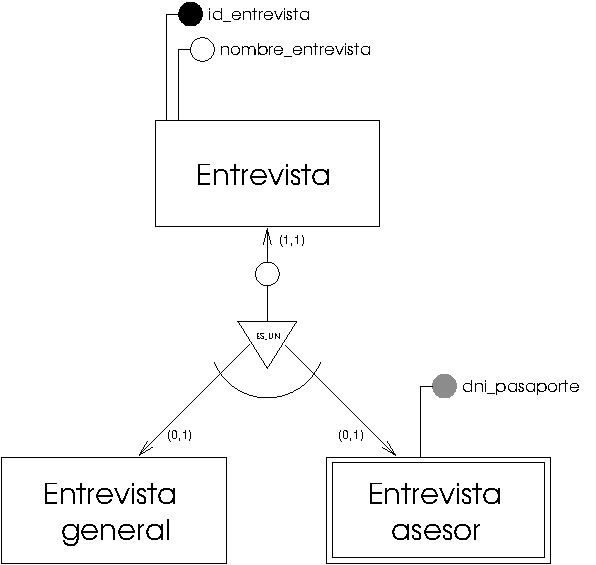
\includegraphics[]{07.Modelo_Entidad-Interrelacion/7.2.Analisis_Entidades/diagramas/entrevista.pdf}
            \caption{Diagrama de la entidad Entrevista.}
            \label{diagramaEntrevista}
            \end{center}
         \end{figure}

   \item[Descripción de los atributos propios] La entidad presenta los
   siguientes atributos propios:

   \begin{itemize}
    \item \textbf{id\_entrevista}
      \begin{itemize}
         \item \textbf{Definición:} Código que sirve como número identificativo
               para cada entrevista del sistema.
         \item \textbf{Dominio:} Números naturales.
         \item \textbf{Carácter:} Obligatorio.
         \item \textbf{Ejemplo práctico:} 24.
         \item \textbf{Información adicional:} El dato lo genera el sistema
               cuando se introduce una nueva entrevista en el sistema. Es la
               clave primaria.
      \end{itemize}
   \item \textbf{nombre\_entrevista}
      \begin{itemize}
         \item \textbf{Definición:} Denominación de una entrevista dentro del
                sistema.
         \item \textbf{Dominio:} Conjunto de caracteres alfanuméricos.
         \item \textbf{Carácter:} Obligatorio.
         \item \textbf{Ejemplo práctico:} Entrevista inicial.
         \item \textbf{Información adicional:} El dato lo introduce el
         administrador principal al introducir una nueva entrevista en el
         sistema.
      \end{itemize}
   \end{itemize}

   \item[Ejemplos prácticos]

   \item \begin{center}
            \begin{tabular}{ | l | l | }
            \hline
            \multicolumn{2}{ | c | }{\textbf{Tipo de entidad Entrevista general}} \\
            \hline
            id\_entrevista & 24 \\
            \hline
            nombre\_entrevista & Entrevista inicial \\
            \hline
            \end{tabular}
         \end{center}

   \item \begin{center}
            \begin{tabular}{ | l | l | }
            \hline
            \multicolumn{2}{ | c | }{\textbf{Tipo de entidad Entrevista asesor}} \\
            \hline
            id\_entrevista & 77 \\
            \hline
            nombre\_entrevista & Entrevista idiomas \\
            \hline
            id\_asesor & 98765432Z \\
            \hline
            \end{tabular}
         \end{center}
   \end{description}
